\section{SQL} 

  SQL (Structured Query Language) is the standard query language supported by most DBMS and is a syntactically sugared form of relational algebra. It is \textbf{declarative}, where the programmer specifies what answers a query should return,but not how the query should be executed. The DBMS picks the best execution strategy based on availability of indices, data/workload characteristics, etc. (i.e. provides physical data independence). It contrasts to a \textbf{procedural} or an \textbf{operational} language like C++ or Python. The reason we need this specific query language dependent on relational algebra is that it is \textit{less} powerful than general purpose languages like C or Python. These things can all be stored in structs or arrays, but the simplicity allows the compiler to make huge efficiency improvements. 

  Just like how we approached relational algebra with structure, operations, and constraints, we will do the same with SQL, although we will introduce structure with constraints first (it's natural to talk about constraints with structure, since you define the constraints when you create the SQL relations). While this wasn't talked about much before, SQL actually uses \textit{multisets}, or \textit{bags}, by default. It's operations support both set and bag operations, and we will cover both of them here. Working with sets or bags is really context dependent, but it does have a few advantages. 
  \begin{enumerate}
    \item To take the union of two bags, we can just add everything into the other without going through to check for duplicates. 
    \item When we project relations as bags, we also don't need to search through all pairs to find duplicates. 
  \end{enumerate}
  This allows for efficiency at the cost of memory. 

\subsection{Structure and Constraints}

    \begin{definition}[Primitive Types]
      The primitive types are listed.\footnote{One thing to note is that keywords are usually written in uppercase by convention.}
      \begin{enumerate}
        \item \textit{Characters}. \texttt{CHAR(n)} represents a string of fixed length $n$, where shorter strings are padded, and \texttt{VARCHAR(n)} is a string of variable length up to $n$, where an endmarker or string-length is used. 
        \item \textit{Bit Strings}. \texttt{BIT(n)} represents bit strings of length $n$. \texttt{BIT VARYING(n)} represents variable length bit strings up to length $n$. 
        \item \textit{Booleans}. \texttt{BOOLEAN} represents a boolean, which can be \texttt{TRUE}, \texttt{FALSE}, or \texttt{UNKNOWN}. 
        \item \textit{Integers}. \texttt{INT} or \texttt{INTEGER} represents an integer. 
        \item \textit{Floating points}. \texttt{FLOAT} or \texttt{REAL} represents a floating point number, with a higher precision obtained by \texttt{DOUBLE PRECISION}. 
        \item \textit{Datetimes}. \texttt{DATE} types are of form \texttt{'YYYY-MM-DD'}, and \texttt{TIME} types are of form \texttt{'HH:MM:SS.AAAA'} on a 24-hour clock. 
        \item \textit{Null}. \texttt{NULL} represents a null value. 
      \end{enumerate}
    \end{definition}
    
    Before we can even query or modify relations, we should know how to make or delete one. 

    \begin{theorem}[\texttt{CREATE TABLE}, \texttt{DROP TABLE}]
      We can create and delete a relation using \texttt{CREATE TABLE} and \texttt{DROP TABLE} keywords and inputting the schema. 
      \begin{lstlisting}
        CREATE TABLE Movies(
          name CHAR(30), 
          year INT, 
          director VARCHAR(50), 
          seen DATE
        ); 

        DROP TABLE Movies; 
      \end{lstlisting}
    \end{theorem}

    \begin{theorem}[\texttt{DEFAULT}]
      We can also determine default values of each attribute with the \texttt{DEFAULT KEYWORD}. 
      \begin{lstlisting}
        ALTER TABLE Movies ADD rating INT 0; 
        ...
        CREATE TABLE Movies(
          name CHAR(30) DEFAULT 'UNKNOWN', 
          year INT DEFAULT 0, 
          director VARCHAR(50), 
          seen DATE DEFAULT '0000-00-00'
        ); 
      \end{lstlisting}
    \end{theorem}

  \subsubsection{Nulls}

    We are not guaranteed that we will have all data. What if there are some null values? We need some way to handle unknown or missing attribute values. One way is to use a default value (like $-1$ for age), but this can mess with other operations, such as getting average values of certain groups of users, or can make computations harder since we have to first filter out users with \texttt{age=-1} before querying. Another way is to use a valid bit for every attribute. For example, \texttt{User(uid, name, age)} could map to \texttt{User(uid, name, name\_valid, age, age\_valid)}, but this is not efficient as well. 

    A better solution is to decompose the table into multiple relations such that a missing value indicates a missing row in one of the subrelations. For example, we can decompose \texttt{User(uid, name, age, pop)} to 
    \begin{enumerate}
      \item \texttt{UserID(uid)}
      \item \texttt{UserName(uid, name)}
      \item \texttt{UserAge(uid, age)}
      \item \texttt{UserPop(uid, pop)}
    \end{enumerate}
    This is conceptually the cleanest solution but also complicates things. Firstly, the natural join wouldn't work, since compared to a single table with null values, the natural join of these tables would exclude all tuples that have at least one null value in them. 

    \begin{definition}[\texttt{NULL}]
      SQL's solution is to have a special value \texttt{NULL} indicating an unknown but not empty value. It has the following properties. 
      \begin{enumerate}
        \item It holds for every domain (null is the same for booleans, strings, ints, etc.). 
        \item Any operations like $+, -, \times, >$... leads to a \texttt{NULL} value. 
        \item All aggregate functions except \texttt{COUNT} return a \texttt{NULL}. \texttt{COUNT} also counts null values. 
      \end{enumerate}
    \end{definition}

    \begin{theorem}[Three-Valued Logic]
      Here is another way to implement the unknown logic with \textit{three-valued logic}. Suppose we set True=1, False=0. Then we can see that given statements $x, y$ which evaluate to $0, 1$, 
      \begin{enumerate}
        \item $x$ and $y$ is equivalent to $\min(x, y)$
        \item $x$ or $y$ is equivalent to $\max(x, y)$ 
        \item not $x$ is equivalent to $1 - x$
      \end{enumerate}
      It turns out that if we set unknown=0.5, then this logic also works out very nicely. Check it yourself. 
    \end{theorem}

    The way operations treat null values is extremely important, and we will add a sentence on how it treats nulls for each operation. 

    \begin{example}[Warnings]
      Note that null breaks a lot of equivalences, leading to unintended consequences. 
      \begin{enumerate}
        \item The two are not equivalent since if we have nulls, the average ignores all nulls, while the second query will sum up all non-nulls and divide by the count including the nulls. 
        \begin{lstlisting}
          SELECT AVG(pop) FROM User; 
          SELECT SUM(pop) / COUNT(*) FROM User; 
        \end{lstlisting}

        \item The two are also not equivalent since \texttt{pop = pop} is not True, but Unknown, for nulls, so it would not return nulls. The first query would return all tuples, even nulls. 
        \begin{lstlisting}
          SELECT * from User; 
          SELECT * from User WHERE pop = pop; 
        \end{lstlisting}

        \item Never compare equality with null, since this never outputs True. Rather, you should use the special keywords \texttt{IS NULL} and \texttt{IS NOT NULL}. 
          \begin{lstlisting}
            SELECT * FROM User WHERE pop = NULL; // never returns anything 
            SELECT * FROM User WHERE pop IS NULL; // correct 
          \end{lstlisting}
      \end{enumerate}
    \end{example}

  \subsubsection{Modifying Tables}

    This was not an operation we defined in relational algebra, but it is so essential that we should state it now. What if we want to add or delete another attribute? This is quite a major change. 

    \begin{theorem}[\texttt{ALTER TABLE}]
      We can add or drop attributes by using the \texttt{ALTER TABLE} keyword followed by 
      \begin{enumerate}
        \item \texttt{ADD} and then the attribute name and then its type. 
        \item \texttt{DROP} and then the attribute name. 
      \end{enumerate}
      \begin{lstlisting}
        ALTER TABLE Movies ADD rating INT; 
        ALTER TABLE Movies DROP director; 
      \end{lstlisting}
    \end{theorem} 

    We have briefly saw how to create and drop tables. To update a table, we can do the following. 

    \begin{definition}[\texttt{INSERT}]
      You can either 
      \begin{enumerate}
        \item insert one row  
          \begin{lstlisting}
            INSERT INTO Member VALUES (789, "Muchang")
          \end{lstlisting} 
        \item or you can insert the output of a query. 
          \begin{lstlisting}
            INSERT INTO Member 
            (SELECT uid, name FROM User); 
          \end{lstlisting}
      \end{enumerate}
    \end{definition}

    \begin{definition}[\texttt{DELETE}]
      You can either 
      \begin{enumerate}
        \item delete everything from a table (but not the schema, unlike \texttt{DROP TABLE}). 
          \begin{lstlisting}
            DELETE FROM Member; 
          \end{lstlisting}

        \item Delete according to a \texttt{WHERE} condition 
          \begin{lstlisting}
            DELETE FROM Member 
            WHERE age < 18; 
          \end{lstlisting}

        \item Delete according to a \texttt{WHERE} condition extracted from another query. 
          \begin{lstlisting}
            DELETE FROM Member 
            WHERE uid IN (SELECT uid FROM User WHERE age < 18); 
          \end{lstlisting}
          
      \end{enumerate}
    \end{definition}

    \begin{definition}[\texttt{UPDATE}]
      You can either 
      \begin{enumerate}
        \item Update a value of an attribute for all tuples. 
          \begin{lstlisting}
            UPDATE User 
            SET pop = (SELECT AVG(pop) from User); 
          \end{lstlisting}

        \item Update a value of an attribute for all tuples satisfying a \texttt{WHERE} condition.\footnote{Note that this does not incrementally update the values. It updates all at once from the average of the old table from the subquery.}
          \begin{lstlisting}
            UPDATE User 
            SET name = 'Barney' 
            WHERE uid = 182; 
          \end{lstlisting}
      \end{enumerate}
    \end{definition}

  \subsubsection{Constraints}

    We mainly use constraints to protect the data integrity and relieve the coder from responsibility. It also tells the DBMS about the data so it can optimize better. 

    \begin{definition}[\texttt{NOT NULL} Constraints]
      This tells that an attribute cannot be entered as null (this is already enforced for keys). 
      \begin{lstlisting}
        CREATE TABLE User 
        (uid INTEGER NOT NULL, 
        name VARCHAR(30) NOT NULL, 
        twitterid VARCHAR(15) NOT NULL, 
        age INTEGER, 
        pop FLOAT); 
      \end{lstlisting}
    \end{definition}

    \begin{definition}[\texttt{PRIMARY KEY}, \texttt{UNIQUE} Key Constraints]
      There are multiple ways to identify keys. 
      \begin{enumerate}
        \item Use the \texttt{PRIMARY KEY} keyword to make \texttt{name} the key. It can be substituted with \texttt{UNIQUE}. You can include at most one primary key, but any number of \texttt{UNIQUE}. This means that either name or id can be used as a key, but we must choose one primary key, so we are restricted to at most one. 
        \begin{lstlisting}
          CREATE TABLE Movies(
            name CHAR(30) NOT NULL PRIMARY KEY,
            id CHAR(30) NOT NULL UNIQUE,
            year INT NOT NULL, 
            director VARCHAR(50), 
            seen DATE
          ); 
        \end{lstlisting}

        \item Use the \texttt{PRIMARY KEY} keyword, which allows you to choose a combination of attributes as the key. It can be substituted with \texttt{UNIQUE}. 
        \begin{lstlisting}
          CREATE TABLE Movies(
            name CHAR(30),
            year INT, 
            director VARCHAR(50), 
            seen DATE, 
            PRIMARY KEY (name, year)
          ); 
        \end{lstlisting}
      \end{enumerate}
    \end{definition}

    \begin{definition}[Referential Integrity]
      Like we said before, a referential integrity means that if an attribute $a$ appears in $R$, then $a$ must appear in some other $T$. That is, there are no \textbf{dangling pointers}, where $R.a$ does exists but $T.a$ does not. There are names for these: 
      \begin{enumerate}
        \item \textbf{Foreign keys} is like $R.a$, where it must point to a valid primary key, e.g. \texttt{User.uid} or \texttt{Group.gid}, which are like entity sets. 
        \item \textbf{Primary keys} are like $T.a$, where it must exist if $R.a$ exists, e.g. \texttt{Member.uid} or \texttt{Member.gid}, which are relationships. 
      \end{enumerate}
      In SQl, we must make sure that the referenced columns must be the primary key and the referencing columns form a foreign key. There are two ways to do it. 
      \begin{lstlisting}
        CREATE TABLE Member (
        uid INT NOT NULL 
          REFERNECES User(uid),  // 1. put the references as you define it
        gid CHAR(10) NOT NULL,   // 2. define the attribute first
        PRIMARY KEY(uid, gid), 
        FOREIGN KEY (gid) REFERENCES Group(gid)); // 2. then reference it
      \end{lstlisting}
      If you have multi-attribute referential integrity, the second method is better. 
      \begin{lstlisting}
        ...
        FOREIGN KEY (gid, time) REFERENCES Group(gid, time)); 
      \end{lstlisting}
    \end{definition}

    \begin{example}[Handling Referential Integrity Violations]
      Say that you have a referential integrity constraint as above. Then there are two scenarios. If we insert or update a Member row so it refers to a non-existent User.uid, the DBMS will not allow this. If we delete or update a User row whose uid is referenced by some Member row, then there are certain scenarios. 
      \begin{enumerate}
        \item \textit{Reject}. The DBMS will reject this. 
        \item \textit{Cascade}. It will ripple changes (on an update) to all referring rows. 
        \item \textit{Set null}. It will set all references to NULL. 
      \end{enumerate}
      These options can be specified in SQL. 
    \end{example}

    \begin{definition}[Tuple/Attribute-Based Checks]
      These checks are only associated with a single table and are only checked when a tuple/attribute is inserted/updated. It rejects if the condition evaluates to False, but \textit{True/Unknown are fine} (unlike only True in \texttt{WHERE} conditions!). There are two ways to write this in SQL. 
      \begin{lstlisting}
        CREATE TABLE User(
          ... // 1. Directly put the check constraint in definition
          age INTEGER CHECK(age IS NULL OR age > 0), 
          ...
        ); 

        CREATE TABLE Member(
          uid INTEGER NOT NULL,           // 2. First define attribute 
          CHECK(uid IN (SELECT uid FROM User)),  // 2. Then check it 
        ...
        )
      \end{lstlisting}
      Note that in the second example, this is sort of like a referential integrity constraint. However, this is weaker since it only checks for changes in the Member relation, while the referential integrity constraint is checked for every change in both the Member and User relations. If a check evaluates to False, then the DBMS rejects the insertions/updates. 
    \end{definition}

\subsection{Basic Relational Algebra Operations} 

  We won't repeat the definitions of the operations as they are mentioned in the first chapter. We will cover SQL syntax for both set and bag operations. Note that the way set operations work in SQL is that they remove duplicates in the operands and then remove duplicates in the result. In bag operations, we can think of each row $a$ having an implicit count of times $c_a$ it appears in the table.  

  \subsubsection{Renaming}
    
    Counterintuitively, the first thing we should know how to do is rename. This is because when we do the rest of these operations, due to naming conflicts, the need to copy a relation, or reduce confusion, we often rename relations and attributes within these queries. 

    \begin{definition}[Renaming]
      There are two ways you can rename an attribute or a relation. 
      \begin{enumerate}
        \item Explicit, using the \texttt{AS} keyword. 
          \begin{lstlisting}
            old_name AS new_name
          \end{lstlisting}
        \item Implicit, using a space. 
          \begin{lstlisting}
            old_name new_name
          \end{lstlisting}
      \end{enumerate}
    \end{definition}

    \begin{example}
      Here's a more informative example, using syntax that we will learn later. Note that by renaming the relation, all attributes are renamed as well. 
      \begin{lstlisting}
        SELECT
            s.id, 
            s.name AS student_name,
            c.name AS course_name
        FROM 
            Students s         -- rename relation
            JOIN Courses c     -- rename relation
            ON s.course_id = c.id; 
      \end{lstlisting}
    \end{example}

  \subsubsection{Set/Bag Operations}

    \begin{definition}[Union]
      The \textbf{UNION} and \texttt{UNION ALL} keywords calculate the set and bag union, respectively. Bag union sums up the counts from the 2 tables. 

      \noindent\begin{minipage}{.5\textwidth}
        \begin{lstlisting}[]{Code}
          (SELECT * FROM Relation1)  // {1, 2, 3}
          UNION 
          (SELECT * FROM Relation2); // {2, 3, 4}
          // {1, 2, 3, 4}
        \end{lstlisting}
        \end{minipage}
        \hfill
        \begin{minipage}{.49\textwidth}
        \begin{lstlisting}[]{Output}
          (SELECT * FROM Relation1)  // {1, 1, 2}
          UNION ALL 
          (SELECT * FROM Relation2); // {1, 2, 2}
          // {1, 1, 1, 2, 2, 2}
        \end{lstlisting}
      \end{minipage} 
      \texttt{UNION} and \texttt{UNION ALL} both treat NULLs as equal to each other. 
    \end{definition} 

    \begin{definition}[Intersection]
      The \textbf{INTERSECT} and \texttt{INTERSECT ALL} keywords calculate the set and bag intersection, respectively. Bag intersection does a proper-subtract\footnote{Subtracts the counts and truncates counts to $0$ if negative. So $\{a, a\} - \{a, a, a\} = \{\}$.} 

      \noindent\begin{minipage}{.5\textwidth}
        \begin{lstlisting}[]{Code}
          (SELECT * FROM Relation1)  // {1, 2, 3}
          INTERSECT 
          (SELECT * FROM Relation2); // {2, 3, 4}
        \end{lstlisting}
        \end{minipage}
        \hfill
        \begin{minipage}{.49\textwidth}
        \begin{lstlisting}[]{Output}
          (SELECT * FROM Relation1)  // {1, 1, 2}
          INTERSECT ALL 
          (SELECT * FROM Relation2); // {1, 2, 2}
          // {1, 2}
        \end{lstlisting}
      \end{minipage}
      Both treat nulls as equal to each other and will return NULL if it appears on both sides. 
    \end{definition}

    \begin{definition}[Difference]
      The \textbf{EXCEPT} and \texttt{EXCEPT ALL} keywords calculate the set and bag difference, respectively. Bag difference takes the minimum of the two counts. 

      \noindent\begin{minipage}{.5\textwidth}
        \begin{lstlisting}[]{Code}
          (SELECT * FROM Relation1)  // {1, 2, 3}
          EXCEPT 
          (SELECT * FROM Relation2); // {2, 3, 4}
        \end{lstlisting}
        \end{minipage}
        \hfill
        \begin{minipage}{.49\textwidth}
        \begin{lstlisting}[]{Output}
          (SELECT * FROM Relation1)  // {1, 1, 2}
          EXCEPT ALL 
          (SELECT * FROM Relation2); // {1, 2, 2}
          // {1}
        \end{lstlisting}
      \end{minipage}
      Both treat NULLs as equal to each other and will return NULL if it appears more times in the first table than the second. 
    \end{definition}

    \begin{example}[Interpretation of Except All]
      Look at these two operations on the schema \texttt{Poke(uid1, uid2, timestamp)}. 

      \noindent\begin{minipage}{.5\textwidth}
      \begin{lstlisting}[]{Code}
        (SELECT uid1 FROM Poke) 
        EXCEPT 
        (SELECT uid2 FROM Poke); 
      \end{lstlisting}
      \end{minipage}
      \hfill
      \begin{minipage}{.49\textwidth}
      \begin{lstlisting}[]{Output}
        (SELECT uid1 FROM Poke) 
        EXCEPT ALL
        (SELECT uid2 FROM Poke); 
      \end{lstlisting}
      \end{minipage}
      The first operation returns all users who poked others but were never poked, while the second returns all users who poked others more than they were poked. 
    \end{example}

  \subsubsection{Predicates, Projection, Selection}

    \begin{definition}[Condition/Predicate]
      The condition $p$ used in in selection and joins is implemented with the \texttt{WHERE} keyword. The operations used in predicates are listed below. 
      \begin{enumerate}
        \item Equality is denoted with \texttt{=}, and not equals is denoted with \texttt{<>}. Equality evaluates to true if both attribute values are not NULL and match.  
        \item Comparisons is done with \texttt{>}, \texttt{<}, \texttt{>=}, \texttt{<=}. 
        \item The \texttt{IN} and \texttt{NOT IN} gives you filters that restrict the domain of a certain attribute. 
        \begin{lstlisting}
          SELECT * 
          FROM relation 
          WHERE sex in ['male', 'female']; 
        \end{lstlisting}
      \end{enumerate} 
      \texttt{WHERE} will only select rows for which the condition is True (not False or unknown). 
    \end{definition}

    Both selection and projection, known as \textbf{queries}, is done with the same keyword \texttt{SELECT}, and we can do both of them at the same time (the DBMS will determine which operation to do first). Unlike set/bag operations before, \texttt{SELECT} is by default a bag operator. 

    \begin{definition}[Selection]
      The \texttt{SELECT \*} and \texttt{SELECT DISTINCT \*} keywords apply the selection bag and set operator, respectively. The $\ast$ species all attributes in the relation. 
      \begin{lstlisting}
        SELECT * 
        FROM relation 
        WHERE 
          p_1 AND p_2 AND ... ; 
      \end{lstlisting}
    \end{definition} 

    \begin{definition}[Projection]
      The \texttt{SELECT} and \texttt{SELECT DISTINCT} keywords apply the projection bag and set operator, respectively. Rather than putting an $\ast$, we should now specify our desired attributes. 
      \begin{lstlisting}
        SELECT date, age, uid
        FROM relation 
      \end{lstlisting}
    \end{definition} 

    \begin{example}[Comparing Null values always returns Null]
      The two are also not equivalent since \texttt{pop = pop} is not True, but Unknown, for nulls, so it would not return nulls. The first query would return all tuples, even nulls. 
      \begin{lstlisting}
        SELECT * from User; 
        SELECT * from User WHERE pop = pop; 
      \end{lstlisting}
    \end{example}

    \begin{example}[Never Compare Equality with Null]
      Never compare equality with null, since this never outputs True. Rather, you should use the special keywords \texttt{IS NULL} and \texttt{IS NOT NULL}. 
      \begin{lstlisting}
        SELECT * FROM User WHERE pop = NULL; // never returns anything 
        SELECT * FROM User WHERE pop IS NULL; // correct 
      \end{lstlisting}
    \end{example}

  \subsubsection{Products and Joins} 

    All products and joins use bag semantics and to use set semantics just use a \texttt{SELECT DISTINCT}. 

    \begin{definition}[Cartesian Product]
      The \texttt{CROSS JOIN} keyword or the \texttt{,} operator is used to calculate the cartesian product of two relations using bag semantics. 
      \begin{lstlisting}
        SELECT *
        FROM table1
        CROSS JOIN table2; 

        SELECT *
        FROM table1, table2; 
      \end{lstlisting} 
    \end{definition}

    \begin{definition}[Theta Join]
      A theta join is performed by simply adding a \texttt{WHERE} clause after a cross join, using bag semantics. 
      \begin{lstlisting}
        SELECT *
        FROM table1, table2 
        WHERE table1.A = table2.B;
      \end{lstlisting}
    \end{definition} 

    \begin{definition}[Natural/Inner Join]
      The \texttt{JOIN} keyword returns records that have matching values in both tables using bag semantics. 
      \begin{lstlisting}[language=SQL]
        SELECT * FROM Students s
        JOIN Courses c ON s.id = c.id;
      \end{lstlisting}
      For inner join, note that NULL attributes do not match each other (as stated in equality predicate) so they are not included. 
    \end{definition}

    \begin{definition}[Left Outer Join]
      \texttt{LEFT (OUTER) JOIN}: Returns all records from the left table $R$, and the matched records from the right table $S$. For a given $r \in R$, if there are no $s \in S$ that matches it, then the $S$ attributes will all be NULL. 
      \begin{lstlisting}[language=SQL]
        SELECT * FROM Students s
        LEFT JOIN Courses c ON s.id = c.id;
      \end{lstlisting} 
      This keeps all NULLs on the left table. 
    \end{definition}

    \begin{definition}[Right Outer Join]
      \texttt{RIGHT (OUTER) JOIN}: Returns all records from the right table $S$, and the matched records from the left table $R$ with potential NULLs. For a given $s \in S$, if there are no $r \in R$ that matches it, then the $R$ attributes will all be NULL. 
      \begin{lstlisting}[language=SQL]
        SELECT * FROM Students s
        RIGHT JOIN Courses c ON s.id = c.id;
      \end{lstlisting}
      This keeps all NULLs on the right table. 
    \end{definition}

    \begin{definition}[Full Outer Join]
      \texttt{FULL (OUTER) JOIN}: Returns all records when there is a match in either left or right table with potential NULLs.
      \begin{lstlisting}[language=SQL]
        SELECT * FROM Students s
        FULL OUTER JOIN Courses c ON s.id = c.id;
      \end{lstlisting}
      This keeps all NULLs on the both tables. 
    \end{definition}

    \begin{example}[Motivation for Outer Join]
      Take a look at the following motivating example. Suppose we want to find all members and their respective groups from \texttt{Group(gid, name)}, \texttt{Member(uid, gid)}, \texttt{User(uid, name)}. Then we can write the query 
      \begin{lstlisting}
        SELECT g.gid, g.name AS gname, 
            u.uid, u.name AS uname 
        FROM Group g, Member m, User u 
        WHERE g.gid = m.gid AND m.uid = u.uid; 
      \end{lstlisting}
      This looks fine, but what happens if \textit{Group} is empty? That is, there is a group in the \textit{Group} relation but does not appear in the \textit{Member} relation. Then, \texttt{m.gid} will evaluate to False and would not appear in the joined table, which is fine, but what if we wanted to make sure all groups appeared in this master membership table? If a group is empty, we may want it to just have null values for \texttt{uid} and \texttt{uname}. In this case, we want to use outer join. 
    \end{example}

    \begin{example}[Complex Example with Beers]
      Given the schemas 
      \begin{enumerate}
        \item \texttt{Frequents(drinker, bar, times\_a\_week)}, 
        \item \texttt{Serves(bar, beer, price)}, 
        \item \texttt{Likes(drinker, beer)}, 
      \end{enumerate}
      say that we want to select drinkers and bars that visit the bars at least 2 times a week and the bars serves at least 2 beers liked by the drinker and count the number of beers served by the bars that are liked by the drinker. The query is shown below. 

      \begin{lstlisting}
        SELECT F.drinker, F.bar, COUNT(L.beer) 
        FROM Frequents F, Serves S, Likes L 
        WHERE F.drinker = L.drinker
          AND F.bar = S.bar 
          AND L.beer = S.beer 
          AND F.times_a_week >= 2 
        GROUP BY F.drinker, F.bar 
        HAVING COUNT(L.beer) >= 2 
      \end{lstlisting}
    \end{example}

\subsection{Arithmetic and Sorting} 

  We can also do arithmetic on columns. 

  \begin{definition}[Arithmetic Operations]
    SQL supports 
    \begin{enumerate}
      \item \textit{Addition} using \texttt{+}. It returns NULL if at least 1 of the operands are NULL. 
      \item \textit{Subtraction} using \texttt{-}. It returns NULL if at least 1 of the operands are NULL. 
      \item \textit{Multiplication} using \texttt{\*}. It returns NULL if at least 1 of the operands are NULL. 
      \item \textit{Division} using \texttt{/}. It returns NULL if at least 1 of the operands are NULL or there is division by $0$ (or may result in error depending on DBMS). For integers it will truncate. 
      \item \textit{Modulo} using \texttt{\%}. It returns NULL if at least 1 of the operands are NULL. 
    \end{enumerate}
    You can use parentheses to compose operations together. 
  \end{definition}

  \begin{example}[Arithmetic]
    Here is a comphrensive example. 
    \begin{lstlisting}
      SELECT 
        price + tax as total_price,
        salary - deductions as net_salary,
        price * quantity as total_value,
        total / count as average,
        id % 2 as is_odd
      FROM Orders; 
    \end{lstlisting}
  \end{example}

  \begin{definition}[Sorting]
    The \texttt{ORDER BY} keyword sorts the relation. In fact, it is more of a display operation since the tuples in the relation are unsorted by definition. 
    \begin{enumerate}
      \item \texttt{ORDER BY attribute ASC} orders in ascending order. This the default. 
      \item \texttt{ORDER BY attribute DESC} orders in descending order.
    \end{enumerate}
  \end{definition}

\subsection{Aggregate Functions} 

    \begin{definition}[Standard SQL Aggregate Functions] 
      \textbf{Aggregate functions} compute something from a collection of tuples, rather than a single row. 
      \begin{enumerate}
        \item \texttt{COUNT} counts the number of rows, including NULLS, in a query. \texttt{COUNT(DISTINCT att)} counts the distinct count of an attribute in a query and ignores NULLs. 
        \item \texttt{SUM} counts the sum of the values of an attribute in a query. It ignores NULL values. 
        \item \texttt{AVG} is the average. It ignores NULL values. 
        \item \texttt{MIN} is the minimum of an attribute. It ignores NULL values and only returns NULL if all values are NULL. 
        \item \texttt{MAX} is the maximum of an attribute. It ignores NULL values and only returns NULL if all values are NULL. 
      \end{enumerate}
    \end{definition}

    \begin{example}[Calculate Popularity within Age Group]
      If we want to find the number of users under 18 and their average popularity, then we can write 
      \begin{lstlisting}
        SELECT COUNT(*), AVG(pop) 
        FROM User 
        WHERE age < 18; 
      \end{lstlisting}
    \end{example}

    \begin{example}[Average is Not Sum/Count]
      The two are not equivalent since if we have nulls, the average ignores all nulls, while the second query will sum up all non-nulls and divide by the count including the nulls. 
      \begin{lstlisting}
        SELECT AVG(pop) FROM User; 
        SELECT SUM(pop) / COUNT(*) FROM User; 
      \end{lstlisting}
    \end{example}

  \subsubsection{Group By} 

    By default, the aggregate function operates on the entire relation. If we want more fine grained control by looking at a subset of tuples, then we can use the \texttt{GROUP BY} clause. 

    \begin{definition}[\texttt{GROUP BY}]
      \texttt{GROUP BY} is used when you want to group the query by equal values of the attributes. The syntax is 
      \begin{lstlisting}
        SELECT ... FROM ... WHERE ... 
        GROUP BY age; 
      \end{lstlisting}
      To parse this, first form the groups based on the same values of all attributes in the group by clause. Then, output only one row in the select clause per group. We can look at the following order
      \begin{enumerate}
        \item \texttt{FROM}. Look at where we are querying from. 
        \item \texttt{WHERE}. Find out if this condition is satisfied to filter the main query. 
        \item \texttt{GROUP BY}. Group rows according to the values of the GROUP BY columns. 
        \item \texttt{SELECT}. Compute the select query for each group. The number of groups should be equal to the number of rows in the final output. 
      \end{enumerate}
      Note that if a query uses aggregation/group by, every column referenced in select must be either aggregated or a group by column. 
    \end{definition}

    \begin{example}
      If we want to find the number of users in a certain age and their average popularity, for all ages, then we can write 
      \begin{lstlisting}
        SELECT age, AVG(pop) 
        FROM Users
        GROUP BY age; 
      \end{lstlisting}
      You don't necessarily have to report the group by attribute in the select. The two following examples are perfectly fine, though in the right query, \texttt{age} may not functionally determine \texttt{AVG(pop)}. 

      \noindent\begin{minipage}{.5\textwidth}
      \begin{lstlisting}[]{Code}
        SELECT AVG(pop) 
        FROM User
        GROUP BY age; 
        
      \end{lstlisting}
      \end{minipage}
      \hfill
      \begin{minipage}{.49\textwidth}
      \begin{lstlisting}[]{Output}
        SELECT age, AVG(pop)  
        FROM User 
        GROUP BY age, name; 
      \end{lstlisting}
      \end{minipage}

      In the example below, this left query is not syntactically correct since \texttt{name} is not in the group by clause or aggregated. This is true even if \texttt{age} functionally determines \texttt{name}. Neither is the right since the lack of a group by clause means that the aggregate query is over the entire relation, which has multiple uid values. 

      \noindent\begin{minipage}{.5\textwidth}
      \begin{lstlisting}[]{Code}
        SELECT age, name, AVG(pop) 
        FROM User
        GROUP BY age; 
      \end{lstlisting}
      \end{minipage}
      \hfill
      \begin{minipage}{.49\textwidth}
      \begin{lstlisting}[]{Output}
        SELECT uid, MAX(pop) 
        FROM User; 
        .
      \end{lstlisting}
      \end{minipage}
    \end{example}

    As you can see, this is great to use for aggregate functions. If there is no group by clause, this is equivalent to grouping everything together.  

    \begin{example}
      Given the relation 

      \begin{table}[H]
        \centering
        \begin{tabular}{|c|c|c|}
          \hline
          \textbf{A} & \textbf{B} & \textbf{C} \\
          \hline
          1 & 1 & 10 \\ 
          2 & 1 & 8 \\ 
          1 & 1 & 10 \\ 
          2 & 3 & 8 \\ 
          2 & 1 & 6 \\ 
          2 & 2 & 2 \\ 
          \hline
        \end{tabular}
        \caption{Original relation. }
        \label{tab:groupby}
      \end{table}
    
      Running the query 
      \begin{lstlisting}
        SELECT A, B, SUM(C) AS S 
        FROM R 
        GROUP BY A, B; 
      \end{lstlisting}
      gives 
      
      \begin{table}[H]
        \centering
        \begin{tabular}{|c|c|c|}
          \hline
          \textbf{A} & \textbf{B} & \textbf{S} \\
          \hline
          1 & 1 & 20 \\ 
          2 & 1 & 14 \\ 
          2 & 3 & 8 \\ 
          2 & 2 & 2 \\ 
          \hline
        \end{tabular}
        \caption{Our query. }
        \label{tab:groupby_output}
      \end{table}
    \end{example}

  \subsubsection{Having} 

    \begin{definition}[\texttt{HAVING}]
      If you want to filter out groups having certain conditions, you must use the \texttt{HAVING} keyword rather than \texttt{WHERE}. The syntax is 
      \begin{lstlisting}
        SELECT A, B, SUM(C) FROM ... WHERE ... 
        GROUP BY ... 
        HAVING SUM(C) < 10; 
      \end{lstlisting}
      You should look at the \texttt{HAVING} clause after you look at the \texttt{GROUP BY} but before \texttt{SELECT}. \texttt{HAVING} will only select rows for which the condition is True (not False or null). 
    \end{definition}

    \begin{example}
      Given the relation 

      \begin{table}[H]
        \centering
        \begin{tabular}{|c|c|c|}
          \hline
          \textbf{A} & \textbf{B} & \textbf{C} \\
          \hline
          1 & 1 & 10 \\ 
          2 & 1 & 8 \\ 
          1 & 1 & 10 \\ 
          2 & 3 & 8 \\ 
          2 & 1 & 6 \\ 
          2 & 2 & 2 \\ 
          \hline
        \end{tabular}
        \caption{Original relation. }
        \label{tab:groupby2}
      \end{table}
    
      Running the query 
      \begin{lstlisting}
        SELECT A, B, SUM(C) AS S 
        FROM R 
        GROUP BY A, B 
        HAVING SUM(C) > 8; 
      \end{lstlisting}
      gives 
      
      \begin{table}[H]
        \centering
        \begin{tabular}{|c|c|c|}
          \hline
          \textbf{A} & \textbf{B} & \textbf{S} \\
          \hline
          1 & 1 & 20 \\ 
          2 & 1 & 14 \\ 
          \hline
        \end{tabular}
        \caption{Our query. }
        \label{tab:groupby2_output}
      \end{table}
    \end{example}

    \begin{example}
      Given the schema \texttt{Sailor(sid, name, age, rating)}, to find the age of the youngest sailor with age at least 18, for each rating with at least 2 sailors, we can run the query. 
      \begin{lstlisting}
        SELECT S.rating, MIN(S.age) AS minage 
        FROM Sailors S 
        WHERE S.age >= 18
        GROUPBY S.rating 
        HAVING COUNT(*) > 1; 
      \end{lstlisting}

      \begin{figure}[H]
        \centering 
        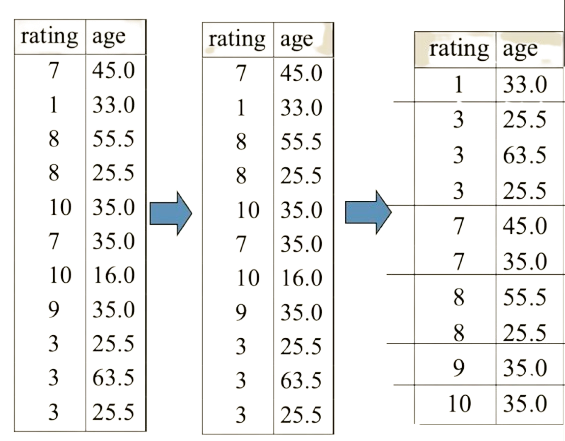
\includegraphics[scale=0.4]{img/sailors.png}
        \caption{The thought process.} 
        \label{fig:thought}
      \end{figure}
    \end{example}

\subsection{Nested Queries and Views} 

  \subsubsection{Subqueries}

    We have so far worked with a single query consisting of a single select statement. However, we can extend this by including queries that have other queries in them. Conceptually, this is easy to understand since we are just composing more operators in relational algebra. 

    \begin{definition}[Subquery]
      A \textbf{subquery} is a query contained inside another query. 
    \end{definition}

    \begin{definition}[Correlated Subqueries]
      A \textbf{correlated subquery} is a subquery that is an input to a parent query. It is a query that needs a parameter from the main query and are generally slower to run. They are hard to parse, but generally you should look in this order (though this is not how the DBMS actually implements it). 
      \begin{enumerate}
        \item \texttt{FROM}. Look at where we are querying from and for loop over each row. 
        \item \texttt{SELECT}. For each row in the outer query, take whatever values/parameters are needed for this row to input into the subquery. 
        \item \texttt{WHERE}. Find out if the condition resulting from the subquery is satisfied. If so, keep this. 
      \end{enumerate}
    \end{definition}

    \begin{definition}[\texttt{EXISTS}]
      The \texttt{EXISTS}(subquery) keyword checks if a subquery is empty or not, and \texttt{NOT EXISTS} checks the negation. 
    \end{definition}

    \begin{example}[Age]
      Given \texttt{User(name, age)}, say that we want to get all users whose age is equal to a person named Bart. Then, we want to select all users from the relation. For each user, we perform the subquery where this original tuple age coincides the others age and the others name is Bart. The outer query only returns those rows for which the \texttt{EXISTS} subquery returned true. Then we can write the two equivalent queries. 

      \noindent\begin{minipage}{.5\textwidth}
      \begin{lstlisting}[]{Code}
        SELECT * 
        FROM User as u
        WHERE EXISTS(SELECT * FROM User
                      WHERE name = "Bart" 
                      AND age = u.age); 
      \end{lstlisting}
      \end{minipage}
      \hfill
      \begin{minipage}{.49\textwidth}
      \begin{lstlisting}[]{Output}
        SELECT * 
        FROM User 
        WHERE age IN(SELECT age 
                      FROM User 
                      WHERE name = 'Bart'); 
      \end{lstlisting}
      \end{minipage}

      To understand this, we use the rules from above. 
      \begin{enumerate}
        \item \texttt{FROM}. We take each row in the outer query. 
        \item \texttt{SELECT}. For each row, we take the age from that row.  
        \item \texttt{WHERE}. The subquery looks for any user named \texttt{Bart} with that same age. If such a user exists, the row is kept. 
      \end{enumerate}
    \end{example}

    Here is a very useful keyword that simplifies complex nested queries, one example of a \textbf{common table expression (CTEs)}. 
    
    \begin{definition}[\texttt{WITH}]
      The \texttt{WITH} clause aliases many relations returned from queries. 
      \begin{lstlisting}
        WITH Temp1 AS (SELECT ...), 
             Temp2 AS (SELECT ...) 
        SELECT X, Y 
        FROM Temp1, Temp2 
        WHERE ...
      \end{lstlisting}
    \end{definition}

    \begin{example}
      To extend the Bart age example, we can think of temporarily storing a query of only Bart's ages, and then comparing it when doing the main query over \texttt{User}. 
      \begin{lstlisting}
        WITH BartAge AS 
          (SELECT age 
          FROM User 
          WHERE name = 'Bart') 
        SELECT U.uid, U.name, U.pop, 
        FROM User U, BartAge B 
        WHERE U.age = B.age; 
      \end{lstlisting}
    \end{example}

  \subsubsection{Scalar Subqueries}
    
    \begin{definition}[Scalar Subqueries]
      Sometimes, if a query returns 1 scalar, then you can use it in your \texttt{WHERE} clause. You must be sure that a query will return exactly 1 scalar (not $0$ and not more than $1$), or there will be a runtime error.  
    \end{definition}

    \begin{example}
      If we want to compute users with the same age as Bart, we can write 
      \begin{lstlisting}
        SELECT * FROM User 
        WHERE age = (SELECT age from User WHERE name = 'Bart'); 
      \end{lstlisting}
      However, we may not know if Bart functionally determines age, so we must be careful. 
    \end{example}

  \subsubsection{Quantified Subqueries}

    \begin{definition}[\texttt{ALL}, \texttt{ANY}]
      We have the following \textbf{quantified subqueries}, which performs a broadcasting condition. 
      \begin{enumerate}
        \item \texttt{ALL} checks if all conditions are true. If any are NULL, then the whole result is NULL. 
        \item \texttt{ANY} checks if any condition is true. If any are true, then the whole result is true. If all are either NULL or false, then \texttt{ANY} will return NULL. 
      \end{enumerate}
    \end{definition}

    \begin{example}[Popular Users]
      Which users are the most popular? We can write this in two ways. 

      \noindent\begin{minipage}{.5\textwidth}
      \begin{lstlisting}[]{Code}
        SELECT * 
        FROM User 
        WHERE pop >= ALL(SELECT pop from User); 
        .
      \end{lstlisting}
      \end{minipage}
      \hfill
      \begin{minipage}{.49\textwidth}
      \begin{lstlisting}[]{Output}
        SELECT * 
        FROM User 
        WHERE NOT 
          (pop < ANY(SELECT pop from User)); 
      \end{lstlisting}
      \end{minipage}

      To review, here are more ways you can do the same query. 

      \noindent\begin{minipage}{.5\textwidth}
      \begin{lstlisting}[]{Code}
        SELECT * 
        FROM User AS u 
        WHERE NOT EXISTS  
          (SELECT * FROM User
          WHERE pop > u.pop); 
      \end{lstlisting}
      \end{minipage}
      \hfill
      \begin{minipage}{.49\textwidth}
      \begin{lstlisting}[]{Output}
        SELECT * FROM User 
        WHERE uid NOT IN 
          (SELECT u1.uid
          FROM User as u1, User as u2 
          WHERE u1.pop < u2.pop); 
      \end{lstlisting}
      \end{minipage}
    \end{example}
  
  \subsubsection{Views}

    \begin{definition}[View]
      A \textbf{view} is a virtual table that can be used across other queries. Tables used in defining a view are called \textbf{base tables}. 
    \end{definition}

    \begin{example}[Jessica's Circle]
      You can create a temporary table that can be used for future queries. 
      \begin{lstlisting}
        CREATE VIEW JessicaCircle AS 
        SELECT * FROM User 
        WHERE uid in (SELECT uid FROM Member WHERE gid = 'jes'); 
      \end{lstlisting}
      Once you are done, you can drop this view with 
      \begin{lstlisting}
        DROP VIEW JessicaCircle; 
      \end{lstlisting}
    \end{example}

\subsection{Recursion} 

  Recursion seems like a foreign concept in relational databases and was not supported until SQL3 , but we can consider the following motivating example. 

  \begin{example}[Ancestors]
    Given a schema \texttt{Parent(parent, child)}, we can find Bart's grandparents with the following query. 
      \begin{lstlisting}
        SELECT p1.parent as grandparent 
        FROM Parent p1, Parent p2 
        WHERE p1.child = p2.parent 
        AND p2.child = 'Bart';
      \end{lstlisting}
      We can do the same for parents, great grandparents, and so forth, but there is no clean way to get all of Bart's ancestors with a single query.  
  \end{example} 

  \begin{definition}[Recursion]
    You can implement a recursive query using the \texttt{WITH RECURSIVE} keyword. 
  \end{definition}

  \begin{example}[Recursive Query for Ancestors]
    Lines 2-7 defines the relation recursively, and then lines 8-10 is the query using the relation defined in the WITH clause. 
    \begin{lstlisting}
      WITH RECURSIVE 
      Ancestor(anc, desc) AS 
      ((SELECT parent, child FROM Parent) -- base case
      UNION 
      (SELECT a1.anc, a2.desc             -- recursion step
      FROM Ancestors a1, Ancestors a2     -- recursion step
      WHERE a1.desc = a2.anc))            -- recursion step
      SELECT anc 
      FROM Ancestor 
      WHERE desc = 'Bart'; 
    \end{lstlisting}
  \end{example}

